\documentclass[50pt]{usiinfbachelorproject}
\captionsetup{labelfont={bf}}
\raggedbottom
\usepackage{graphicx}
\usepackage{listings}
\usepackage{float}
\usepackage{titlesec}
\usepackage{subfigure}

\lstnewenvironment{code}{\lstset{language=Python}}{}

\setlength{\parskip}{5pt}


\titleformat{\paragraph}
{\normalfont\normalsize\bfseries}{\theparagraph}{1em}{}
\titlespacing*{\paragraph}
{0pt}{3.25ex plus 1ex minus .2ex}{1.5ex plus .2ex}

\author{Harkeerat Singh Sawhney}

\title{A Comparative Study between Google and Conversational AI Models}

\versiondate{\today}

\begin{committee}
%With more than 1 advisor an error is raised...: only 1 advisor is allowed!
\advisor[Universit\`a della Svizzera Italiana, Switzerland]{Prof.}{Landoni}{Monica}

\end{committee}

\abstract {
    The ubiquitous nature of the internet has led to a surge in online activity among young children, making it a go-to source for information. However, the reliability and accuracy of online information tend to be often questioned, particularly for children who are unaware of its veracity. Recently, there has been a much more user-friendly approach to accessing online information in the form of Conversational AI Models. The thesis would draw a comparative analysis between Google Search and Conversational AI models such as ChatGPT, to determine the more effective option in the context of Children’s online search behavior. The study would make use of innovative tools to simplify the comparison between ChatGPT and Google Search, aiming to identify the technology that yields superior outcomes. Along with that this thesis also includes the development of modules to predict the relevance of query results which can be used to determine whether search query outcomes are pertinent or not. Finally, with the goal of improving the quality of information available to young children, this study aims to contribute to the field of online search behavior research.
}

 
{\fontsize{20}{16}\selectfont
% your selected code here

\begin{document}
\maketitle
\tableofcontents

\newpage
\listoffigures
\listoftables

\newpage

%%%%%%%%%%%%%%%%%%%%%%%%%%%%
\section{Introduction}
The increasing accessibility of the internet has revolutionized the way young children access information. With the advent of online resources, children now have access to a vast amount of information. However, on the other hand, online information \cite{slone2003internet} is often met with skepticism due to the potential unreliability and inaccuracy of the sources. Along with that, young children are often unaware of how to identify credible sources of information, which can lead to a significant impact on their knowledge acquisition.

In recent years, conversational AI models such as ChatGPT have emerged as a user-friendly way of accessing online information. Such models have allowed users to converse with the machine in a natural language format, which can be particularly effective for children. Still, skepticism stays, as to if such conversational AI models improve on the problems that traditional searching methods have introduced, or does it make it worse due to the generative nature of such models.

\subsection{Structure of the Thesis}
This thesis report will follow the sequential procedure of the project, which will start from the inception to the end of the project. Section \ref{sec:background} contains the background and motivation of the project, which will include the fundamental concepts of Information Pollution and Hallucination. It will also include the impact of such phenomena on children and how it affects them as they are the primary focus of this research. This section will also introduce the two technologies which we are going to compare; ChatGPT and Google Search. At the end of this section, some literature work would be mentioned which is written in the same field and would give better insight into the subject.

Section \ref{sec:methodology} will focus on the methodology of the project, which will include in detail the different steps which were taken in order to collect the data, how the data was pre-processed, and how it was used to have different analyses done one it with different metrics. There were many different types of metrics used ranging from multiple different similarity analyses to sentiment analysis. The main reason for this was to have a robust analysis of the data which was collected.

Section \ref{sec:machine_learning_model} will utilize the data collected and would aim to develop a machine-learning model which can predict the relevance of the query results. The model would be trained on the collected data while utilizing various different machine-learning techniques. 

Finally Section \ref{sec:validation} will conclude the thesis by discussing what all the results mean and as to which technology is better for children to use right now. It will also discuss the limitations of the project and would describe directions for future work.

At last all of the work which was done in this thesis would be available on GitHub \footnote{
\url{https://github.com/Harkeerat2002/bachelor-project-scripts }}. The GitHub repository contains all the scripts which were developed throughout the project and also contains the data which was collected. It also contains all the results which were obtained from the analysis of the data. There is robust documentation available on the repository which would help anyone who wants to replicate the results or wants to use the scripts for their own use.

\section{Background and Motivation}
\label{sec:background}

\subsection{Information Pollution and Hallucinations}
As of today one of the major challenges in surfing on the internet is Information Pollution \cite{pandita2014information}. Information Pollution is the contamination of the information supply with irrelevant, redundant, unsolicited, hampering, and low-value information. Information Pollution is caused due to the overwhelming and excessive amount of information, which is often of low quality. Such information often circulates through many different communication channels, especially on search engines. This can cause long-lasting damage to those who receive such incorrect and distracting information, as it causes affects their knowledge and as well their quality of life.

There are many different forms in which Information Pollution can be presented. One such form is misinformation \cite{meel2020fake}, which is caused by inaccurate information which is shared with each other in an attempt to deceive. Another form of which information pollution can be present is disinformation, which, unlike misinformation, is deliberately fabricated to mislead people. As it can be noticed many times the origin of such information is malicious, however, due to the nature of the internet, they are very easily shared amongst everyone without being checked. 

Another form in which Information Pollution can be present is Hallucinations \cite{shuster_poff_chen_kiela_weston_2021}. Hallucinations in information technology tend to present significant challenges in various domains, ranging from user interface design to more recently artificial intelligence systems. Such hallucinations are instances where users tend to perceive or experience inaccurate, misleading, or irrelevant information, which tends to erroneous decision-making and compromised user experience. Such phenomena usually can arise to factors such as limitations in data quality, algorithmic biases, and inefficiencies in information retrieval systems.

\subsection{Children's Search Behavior}
As much as it is challenging for adults to tackle Information Pollution, it is much more difficult for children to tackle it. One of the primary victims of Information Pollution is children, as Information Pollution expose their vulnerability regarding their developing cognitive abilities. Children can come across false or misleading information, which can lead to the formation of misconceptions and incorrect beliefs regarding various subjects \cite{lovenheim2018does}. This can be very harmful as it can hinder their understanding of the world and have a negative impact on making informed decisions. Another factor that can affect children is their development of Critical Thinking Skills \cite{kalinina2018psychological}. If children are having constant exposure to Information Pollution, it can make it challenging for children to develop critical thinking skills. Children can struggle to discern reliable sources of information, evaluate their credibility and differentiate between a fact and an opinion. 

Along with that Hallucination poses an additional challenge for children in Information Retrieval \cite{shuster_poff_chen_kiela_weston_2021}. This again is challenging for Children to tackle, as hallucinations tend to take advantage of children. One of the main factors which are harmful to children is misinformation and false beliefs. Children rely on search engines or online platforms for information, hence hallucinations in the search results can lead to the dissemination of inaccurate or false information. This could possibly lead to children shaping their understanding of the world around them with misconceptions or false information. This also causes another side effect, which is that it can force children to develop Cognitive Biases with distorted perspectives. Children are still developing their critical skills, and if hallucination is presented in the search results it can lead to them accepting biased, or misleading information as factual.

\subsection{ChatGPT vs Google Search}
The primary method for getting information for a long time has been Google Search \cite{hillis2012google}. It is a web search engine which is developed by Google, one of the world’s leading technology companies. Its purpose is to help users find information on the internet by providing a list of relevant web pages, documents, images, videos, and other types of content in response to their search queries. In order to provide the most appropriate search results it takes various factors into account to determine their relevance and the rankings. These factors include the keywords and language used in the query and its popularity and the quality of the web pages. This makes powerful use of Google’s algorithm which helps with the evaluation of the web pages. This is powered by the web crawlers which explore the web to regularly find pages to add to their index. Along with all the core web search functionalities, Google Search also offers various specialized search features, such as image search, news search, video search, and more. 

However, with the recent advancements in the field of Natural Language Processing, conversation AI models have become much better at providing relevant information with their robust model. One such model is ChatGPT \cite{firat2023chat}, which has been very popular recently. The product is rather very simple to use, there is a text box where the user can type in their questions and from that question, ChatGPT would generate a response. The response is generated by the model by taking into account the context of the question and also the previous question. This makes it very easy for the user to get the information they want.

While ChatGPT does provide very useful information and acts as an assistant, Google Search does also provide more types of media as a result. Therefore, it is important to compare the two technologies and see which one is better for children to use. This is important as it would help us understand which technology is better for children to use and which one is more prone to Information Pollution and Hallucinations.

\subsection{Literature Review on related work}
To get a better understanding of such a topic we went through several different literatures which went into detail with topics such as ChatGPT and Information Pollution. The main aim of reading such literature was to modify our project and seek where there is still some research needed. Out of the many different papers which were read, there were two papers which were very helpful.

The first paper is titled \textit{“What Is the Impact of ChatGPT on Education? A Rapid Review of the Literature”} \cite{lo2023impact}. This paper goes in-depth about the performance and application of ChatGPT in various fields such as economics, programming, mathematics, etc. Their finding stated that although ChatGPT has a very strong potential to serve as an assistant for instructors, it still is a challenge as it can generate incorrect information. Also, even though in fields like programming ChatGPT’s performance was satisfactory, it performed very poorly in other fields such as mathematics.  

The second paper which we went through is titled \textit{“On the Risk of Misinformation Pollution with Large Language Models”} \cite{pan2023risk}. This paper does a comprehensive investigation into the potential misuse of modern Large Language Models for the generation of credible-sounding information. The paper discusses how it established a model which simulates potential misuse scenarios so that they can assess how LLMs utilize the produced misinformation. Their initial results showed that there are trends of defensive strategies, and it was concluded that much more work needs to be still done for the challenge of misinformation pollution. 

Overall, these 2 papers highlight the presence of ChatGPT in the landscape of gaining information in the modern world. It highlights the possible threats that ChatGPT can cause but also states that its potential is good enough to risk those threats. 

\subsection{Research Questions and Objectives}
Hallucination and Information Pollution can be mitigated by giving essential education to children about critical evaluation and information sources and encouraging them to seek guidance from trusted sources. However, these days with conversation systems powered by artificial intelligence the line between trustworthy information and compromised information is disappearing day by day. Even adults are more likely to mistake what a trustworthy source is, so not much can be expected from children. Therefore, the question arises, are the new conversations AI models safer for children to interact with, or do the traditional search engine still hold an edge over the new technology?

Hence, this thesis will aim to identify between ChatGPT and Google Search, which offers the best overall service to children, so as to present the least Information Pollution and Hallucination in the results it provides. The study will first collect queries from children and will perform different analyses on them. In the end, the goal is to also make a logistic regression-based machine learning module trained on the data which is collected. This is to determine if the information gathered either from ChatGPT or Google Search is relevant or not. At last, finally, the objective is to give a practical conclusion as to at this point what is a better service to utilize for children. 




\section{Methodology}
\label{sec:methodology}
\subsection{Data Collection}
To collect data from Google Search and ChatGPT, the initial step is to collect data directly from children. More specifically data is needed derived from search queries that children use on day-to-day bases to search online. This task presents certain challenges as it necessitates not only organizing and allocating time for the children but also creating a comfortable environment where they feel at ease. Considering these factors, it was decided to utilize pre-existing data that have been previously collected from children under the guidance of Professor Landoni Monica and her team, how collected ethical approval from the school where the study took place originally. Even though the data is old, it is still believed that it is not old enough to be considered outdated. A total of 77 queries were collected, which is a healthy size for data collection to be used for this explorative study. Table \ref{tab:example} shows a sample of the queries that were collected.

\noindent
\begin{table}[H]
  \centering
  \begin{tabular}{|c|l|}
    \hline
    Query Number & Query \\
    \hline
    \hline
    1 & when was the last time capulin erupted \\
    \hline
    2 & what year did the Capulin Volcano in New Mexico Last errupt \\
    \hline
    3 & what year did the Capulin Volcano Last errupt \\
    \hline
    4 & in Arizona what dessert is the Organ Pipe Cactus Monument found in \\
    \hline
    5 & in Arizona what dessert is the Organ Pipe Cactus Monument in Arizona found \\
    \hline
    ... & .... \\
    \hline
    ... & .... \\
    \hline
    ... & .... \\
    \hline
    77 & pictures of hawaii\\
    \hline
  \end{tabular}
  \caption{Queries collected from Children}
  \label{tab:example}
\end{table}

\subsubsection{Google Search}
In order to collect the query results from Google, Google’s own API known as Google Search API was used. Google Search API or officially known as Google Custom Search JSON API, allows us to use Google’s Search functionally. Through this, the results can be retrieved in a JSON format which can then be used to easily do analysis on them. In order to retrieve the results the following steps were taken.

\begin{enumerate}
  \item textbf{Obtaining an API Key:} \\
  There are 2 keys that are needed to get the results from Google Search. The first key is the API key itself, which is used to authenticate the request to the API. The second key is the SEARCH ENGINE KEY which is used to identify the specific search engine which it wanted to be 
  \item \textbf{Constructing a Search Request:} \\
  \noindent
  \begin{minipage}{\linewidth}
  \centering
  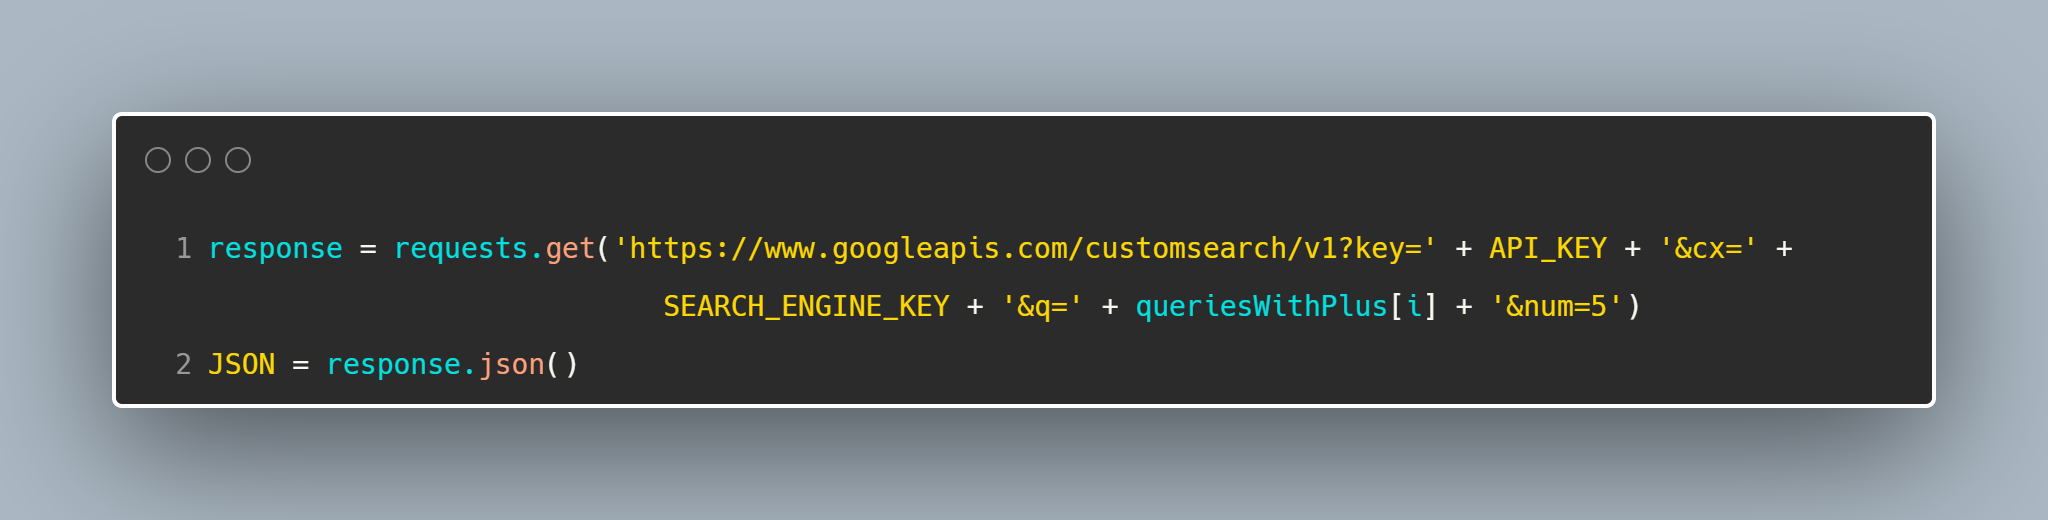
\includegraphics[width=0.9\textwidth]{images/google-search-configuration.png}
  \captionof{figure}{Google Search Configuration}
  \label{fig:google-search-configuration}
  \end{minipage}
  \\
  To send the request, we first need to construct the Search Request which would be sent. The search request has 5 main factors in it. Those are Base URL, API Key, Search Engine ID, Search Query, and Number of Search results. The base URL is the standard URL to use the Google Custom Search API, the API key is used for the authentication, the Search Engine ID is used to specify the engine, Search Query is the query itself from which we want the results and finally, the number of queries is the number of results we want, we have kept to 5. The figure below is the visual representation of what the search request looks like.

  \item \textbf{Sending the Request:}\\
  Finally, the requests are sent, and the data is collected. The data is collected in a JSON which gets processed later. However, with the free plan, we can only send 100 requests per day. So in case there is some bug, either a new API key needs to be generated or we have to wait for a day.
  \item \textbf{Processing the Response:}\\
  At last, the data is received initially in a JSON format, as it is easier to handle the data in that format. However, the JSON data is converted to CSV for consistency, so it is easy to read the data and visualize it with easier tools and libraries.

\end{enumerate}
\subsubsection{ChatGPT}
In order to collect data from ChatGPT, Open AI’s API was used to accomplish this. First, the API key was obtained, and after that the request was configured. In the configuration, there were multiple options, but all the options were configured in such a way that it acts fully as ChatGPT. After that, a request was sent for each of the queries. Unlike Google, for each of the search queries, only one response is generated, as unlike Google where at a time one can see multiple snippets of the results, here only one response is generated at a time. The following were the steps taken with more details describing them.



\begin{enumerate}
  \item \textbf{Obtaining the OpenAI API Key:} \\
  In order to use ChatGTP, naturally an API key is required from Open AI. That can be accessed by making the account and registering for the key. One thing which must be kept in mind is the price of the key since it uses tokens, and each token has a different price range.
  \item \textbf{Configuring the ChatGPT Model:} \\
  \noindent
  \begin{minipage}{\linewidth}
  \centering
  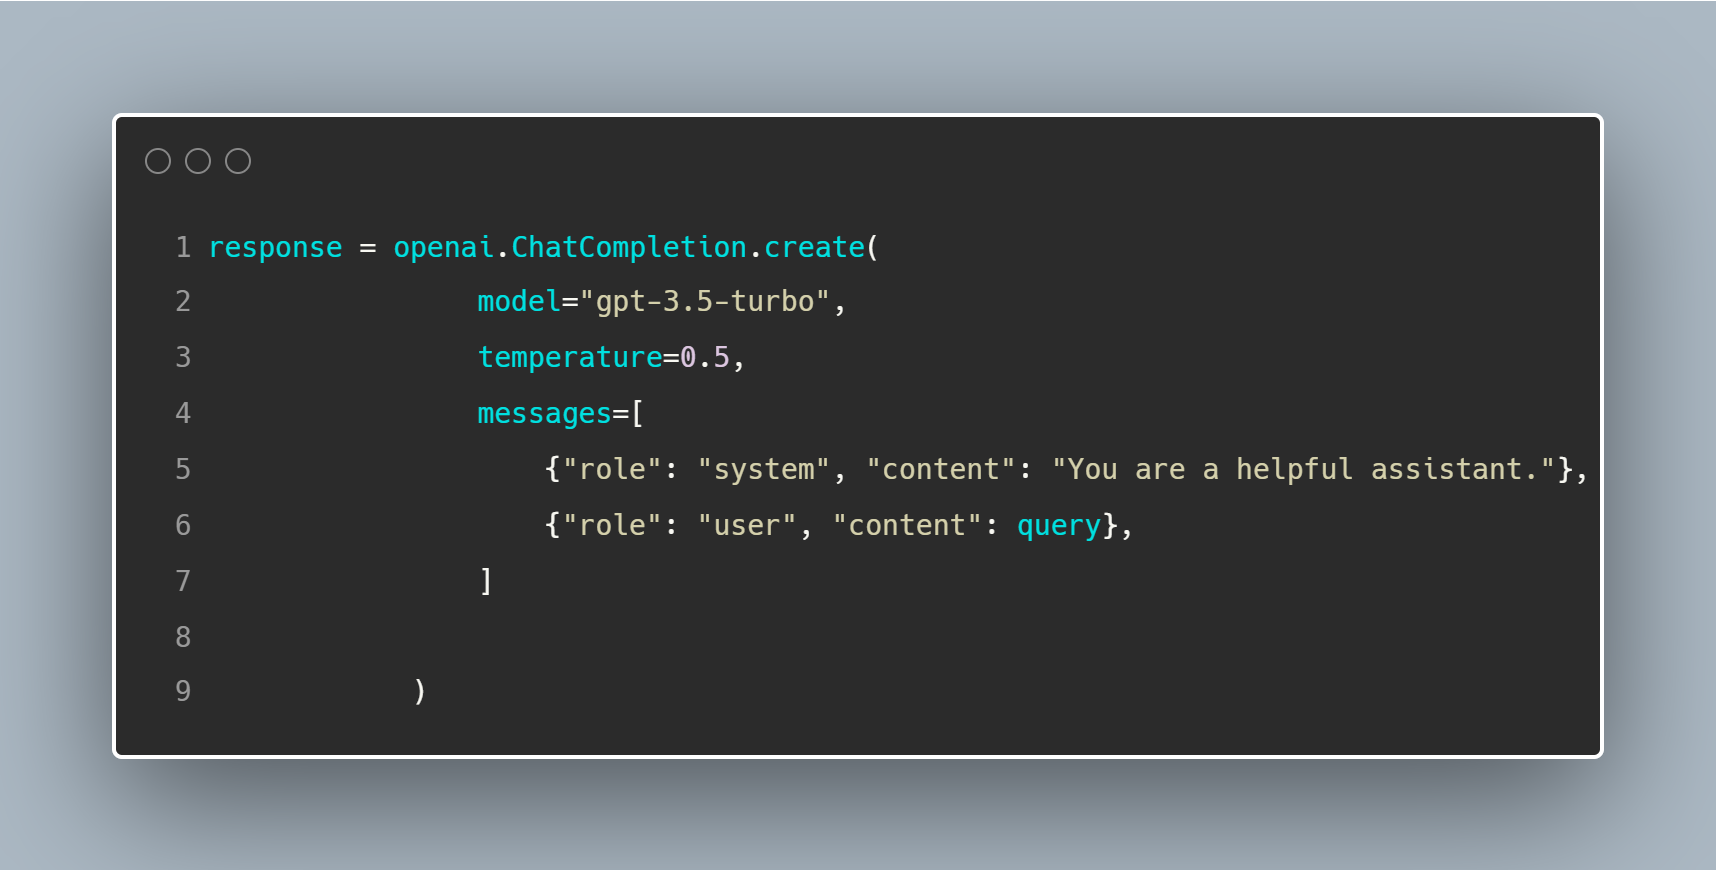
\includegraphics[width=0.6\textwidth]{images/chatgpt-configuration.png}
  \captionof{figure}{ChatGPT Configuration}
  \label{fig:chatgpt-configuration}
  \end{minipage}
  \\
  Open AI gives multiple options to configure what kind of request is needed. In our case, the model which is used is the gpt-3.5-turbo which at the time was the bleeding edge engine that Open AI offered. Also, the temperature value was configured to default which is 0.5. The temperature value controls the creativity of ChatGPT, the higher the value the more creative it gets; however, we want to the standard which is why it was kept to 0.5. At last, the role of ChatGPT was configured. There is an option that we have access to, called a message parameter, which is a list of dictionaries representing the messages in the chat session. Each dictionary contains 2 keys. The first key is “roles”, which tends to specify whether the message is from the user or the system. The second key is “content” which contains the content of the text message. In our case, there were 2 messages which were sent. One was from the system stating, “You are a helpful assistant”, and the second message was from the user stating the query from those collected from children. This configuration can be seen in Figure \ref{fig:chatgpt-configuration}, which was used to configure the request.
  \item \textbf{Sending the Request:} \\
  At last, the request is sent and retrieved in a JSON format. There is no bottleneck that was found with OpenAI as Google, so the procedure was very straightforward.
  \item \textbf{Processing the Response:} \\
  At last, the data is received initially in a JSON format, as it is easier to handle the data in that format. However, the JSON data is converted to CSV for consistency, so it is easy to read the data and visualize it with easier tools and libraries.
\end{enumerate}
\subsection{Data Preprocessing}
This is a crucial step for the next sections Data Analysis and Machine Learning, as using the raw data could cause many inconsistencies. It is important to transform the data in a formal which can be then easily analyzed and be used with different algorithms. The main goal is to improve the quality of the data and make it more suitable for our project. 

What we have done is, we have taken the results from Google and ChatGPT and processed them to create a list of dictionaries that contains the user queries and an array of results. For Google results, the array of results has 5 results in them (the first five returned), while for ChatGPT it has only one result in them. Also, in some cases of Google Results, there were characters that were not needed and had no use of them in the actual analysis. These results were converted from CSV to JSON, from which algorithms such as Sentiment Analysis, Similarity Analyses, and Machine Learning Model were used for their purpose.

\subsection{Data Analysis}
\subsubsection{Query Length Analysis}
The main purpose of the Query Length Analysis \cite{arampatzis2008study} was to compare the length of the responses from both Google Search and ChatGPT. The main purpose of this analysis is to see which one gives more text. Having more text could have several advantages such as much more detailed and comprehensive information related to the topic being searched on. However, they are also several disadvantages to this as well, such as the information can be overwhelming and reading and assessing it can be very time-consuming. \\

\noindent
\begin{minipage}{\linewidth}
\centering
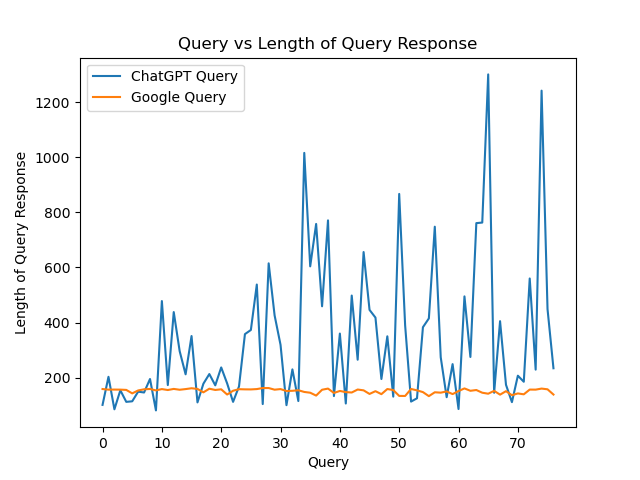
\includegraphics[width=0.9\textwidth]{images/length-of-snippet.png}
\captionof{figure}{ChatGPT Query Length vs Google Search Query Length}
\label{fig:snippet-length}
\end{minipage}

From Figure \ref{fig:snippet-length} we can see that Google and ChatGPT have big differences in terms of the length of their results. Google results in average length is around 151 characters and as compared to ChatGPT its average results length is 343 characters, more than twice as compared to Google results. However, Google Results tends to be more consistent with its query length, as the max is 162 characters and the min is 132 characters. On the other hand, the max for ChatGPT is 1321 characters, while the min goes as low as 81 characters. Table \ref{table:query-length-analysis} is representing the findings.

\begin{table}[H]
  \centering
  \begin{tabular}{|c|c|c|}
    \hline
    & Google Search & ChatGPT \\
    \hline
    \hline
    Average (Characters) & 151 & 343 \\
    \hline
    Max (Characters) & 162 & 1321 \\
    \hline
    Min (Characters) & 132 & 81 \\
    \hline
  \end{tabular}
  \caption{Query Length Analysis}
  \label{table:query-length-analysis}
\end{table}

With this there are several findings, such as ChatGPT results length can vary depending on what question is being asked. This is a good experience as it can identify which topics need more explanation and which need less. However, it can also lead to more information pollution in the text if it tries to generate more. On the other hand, Google results tend to stay consistent with its length, which could mean that for some results it does not provide more details, however, it also can possibly mean that whatever it is providing is more likely relevant as compared to ChatGPT.


\subsubsection{Named Entity Recognition (NER)}
Named Entity Analysis \cite{mikheev1999named} is a natural language processing technique that involved identifying and classifying named entities in text into different predefined categories. For example, such categories can be a person, names, organization names, locations, dates, and so on. This analysis can help us judge how much important information a response contains. The more it contains, we could use it as a factor to conclude the more relevant information it has. Table \ref{tab:entity_categories} is a representation of all the categories which is contained in the Named Entity Analysis

  

\begin{table}[H]
  \centering
  \begin{tabular}{|c|l|}
    \hline
    Categories & Description \\
    \hline
    \hline
    Person & Refers to individuals, including their names, titles, and professions. \\
    \hline
    Organization & Refers to companies, institutions, and other organizations, including their names and types. \\
    \hline
    Location & Refers to places, including countries, cities, and other geographical locations. \\
    \hline
    Date & Refers to specific dates or date ranges, including days, months, years, and seasons. \\
    \hline
    Time & Refers to specific times or time ranges, including hours, minutes, and seconds. \\
    \hline
    Money & Refers to monetary values, including currencies, amounts, and units of measurement. \\
    \hline
    Percentage & Refers to percentages, including numerical values and units of measurement. \\
    \hline
    Product & Refers to products, including their names and types. \\
    \hline
    Event & Refers to specific events, including their names and types. \\
    \hline
    Miscellaneous & Refers to other named entities that do not fit into the above categories. \\
    \hline
  \end{tabular}
  \caption{Named Entity Analysis Categories}
  \label{tab:entity_categories}
\end{table}

To start the analysis, we first need the en-core-web-sm model, which is a pre-trained statistical model for natural language processing. It is part of the spacy library which is a popular open-source library for NLP in Python. For each of the responses of ChatGPT and Google, we use the NLP object to perform the NER and to write the results to the output file. It does this by tokenizing the text into individual words and assigning part-of-speech tags to each word. We can then use the metadata for each word to associate NLP tasks, in which in our case we are naming each entity.

\noindent
  \begin{minipage}{\linewidth}
  \centering
  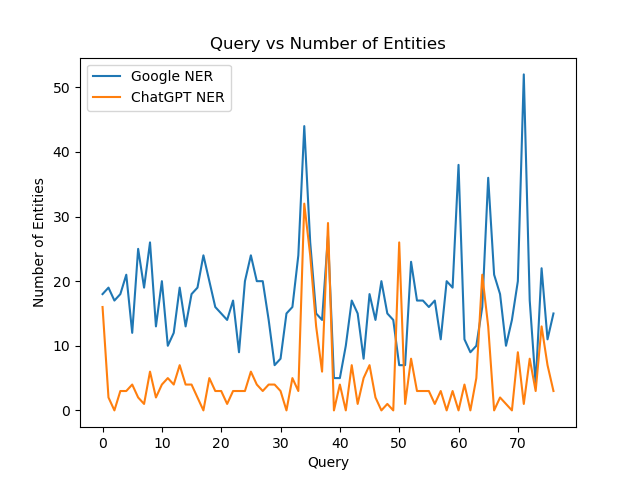
\includegraphics[width=0.9\textwidth]{images/number-of-entities.png}
  \captionof{figure}{Named Entity Analysis}
  \label{fig:name-entity-analysis}
  \end{minipage}
  \\

When looking at the statistical analysis, the average entity is much higher for Google Results. Google has an average of 18.2 entities for each search, while ChatGPT has an average of 6.11, nearly 3 times less as compared to Google. There can be some reasons for this, such as Google results giving out 5 results as compared to ChatGPT giving out one generate result.
  
When it comes to seeing what the top 5 entities are can be seen that ORG, GPE, CARDINAL and PERSON are in the top 5 for both Google Search and ChatGPT. However, the only 2 different entities which aren’t present in the top 5 are DATA (present in Google) and LOC (present in ChatGPT). Table \ref{table:entity-analysis} has all the statistical analysis for the Named Entity Analysis.

\begin{table}[H]
  \centering
  \begin{tabular}{|c|c|c|}
    \hline
    & Google Search & ChatGPT \\
    \hline
    \hline
    Average & 18.2 & 6.11 \\
    \hline
    Max & 35 & 17 \\
    \hline
    Min & 8 & 1 \\
    \hline
  \end{tabular}
  \caption{Named Entity Analysis}
  \label{table:entity-analysis}
\end{table}

\begin{table}[H]
  \centering
  \begin{tabular}{|c||c|c|c|c|c|}
    \hline
    Entity & DATE & ORG & GPE & PERSON & CARDINAL \\
    \hline
    Occurrences & 304 & 237 & 236 & 227 & 211 \\
    \hline
  \end{tabular}
  \caption{Top 5 Google Entities}
  \label{table:top-5-google-entity}
\end{table}

\begin{table}[H]
  \centering
  \begin{tabular}{|c||c|c|c|c|c|}
    \hline
    Entity & GPE & ORG & CARDINAL & PERSON & CARLOCDINAL \\
    \hline
    Occurrences & 108 & 105 & 71 & 49 & 30 \\
    \hline
  \end{tabular}
  \caption{Top 5 ChatGPT Entities}
  \label{table:top-5-google-entity}
\end{table}


\subsubsection{Similarity Analysis}
Similarity Functions are mathematical functions that measure the similarity between two objects or data points. The functions take input data and produce a numerical score that reflects how similar or dissimilar those objects are. In the context of our research, we can use this method of analysis to compare how similar or how dissimilar are Google Search and ChatGPT results. This data could be very helpful with the context of other data when combined, which can help us give meaningful results. We will be using 4 different Similarity Functions which are Cosine Similarity, Jaccard Similarity, Euclidean Similarity, and Pearson Similarity. The data when finally collected is represented in a CSV as the below table represents. Table \ref{tab:similarity_analysis_data_structure} shows the data structure of the Similarity Analysis.

\begin{table}[H]
  \centering
  \begin{tabular}{|c|c|c|c|c|c|c|}
    \hline
    User Query & ChatGPT Result & Google Result & Jaccard & Cosine & Euclidean & Pearson\\
    \hline
    \hline
    ... & .... & .... & .... & .... & .... & .... \\
    \hline
  \end{tabular}
  \caption{Similarity Analysis Data Structure}
  \label{tab:similarity_analysis_data_structure}
\end{table}
\paragraph{Cosine Similarity}
Cosine Similarity \cite{dehak2010cosine} is a measure of similarity between two non-zero vectors defined in an inner product space. It is the measurement of the cosine of the angle between the vectors, which is the dot product of the vectors divided by the product of their lengths. Along with that Cosine Similarity also shows that it does not depend on the magnitudes of the vectors but on its own vectors. The Cosine Similarity gives a value which is between -1 and 1. 1 indicates that the two vectors being compared are identical, while 0 indicates that the two vectors are orthogonal (have no correlation), and -1 indicates that the two vectors are diametrically opposed.

In our case where we are processing the information, each word is assigned a different coordinate. Then the document is represented by the vectors of the number of occurrences of each word in the document. With this, we can judge how similar the documents are. Hence, the cosine of two non-zero vectors can be derived by using the Euclidean Dot Product Formula.

\begin{align}
  A \cdot B &= \|A\| \|B\| \cos(\theta) \\
  \cos(\theta) &= \frac{A \cdot B}{\|A\| \|B\|}
\end{align}

  \noindent
  \begin{minipage}{\linewidth}
  \centering
  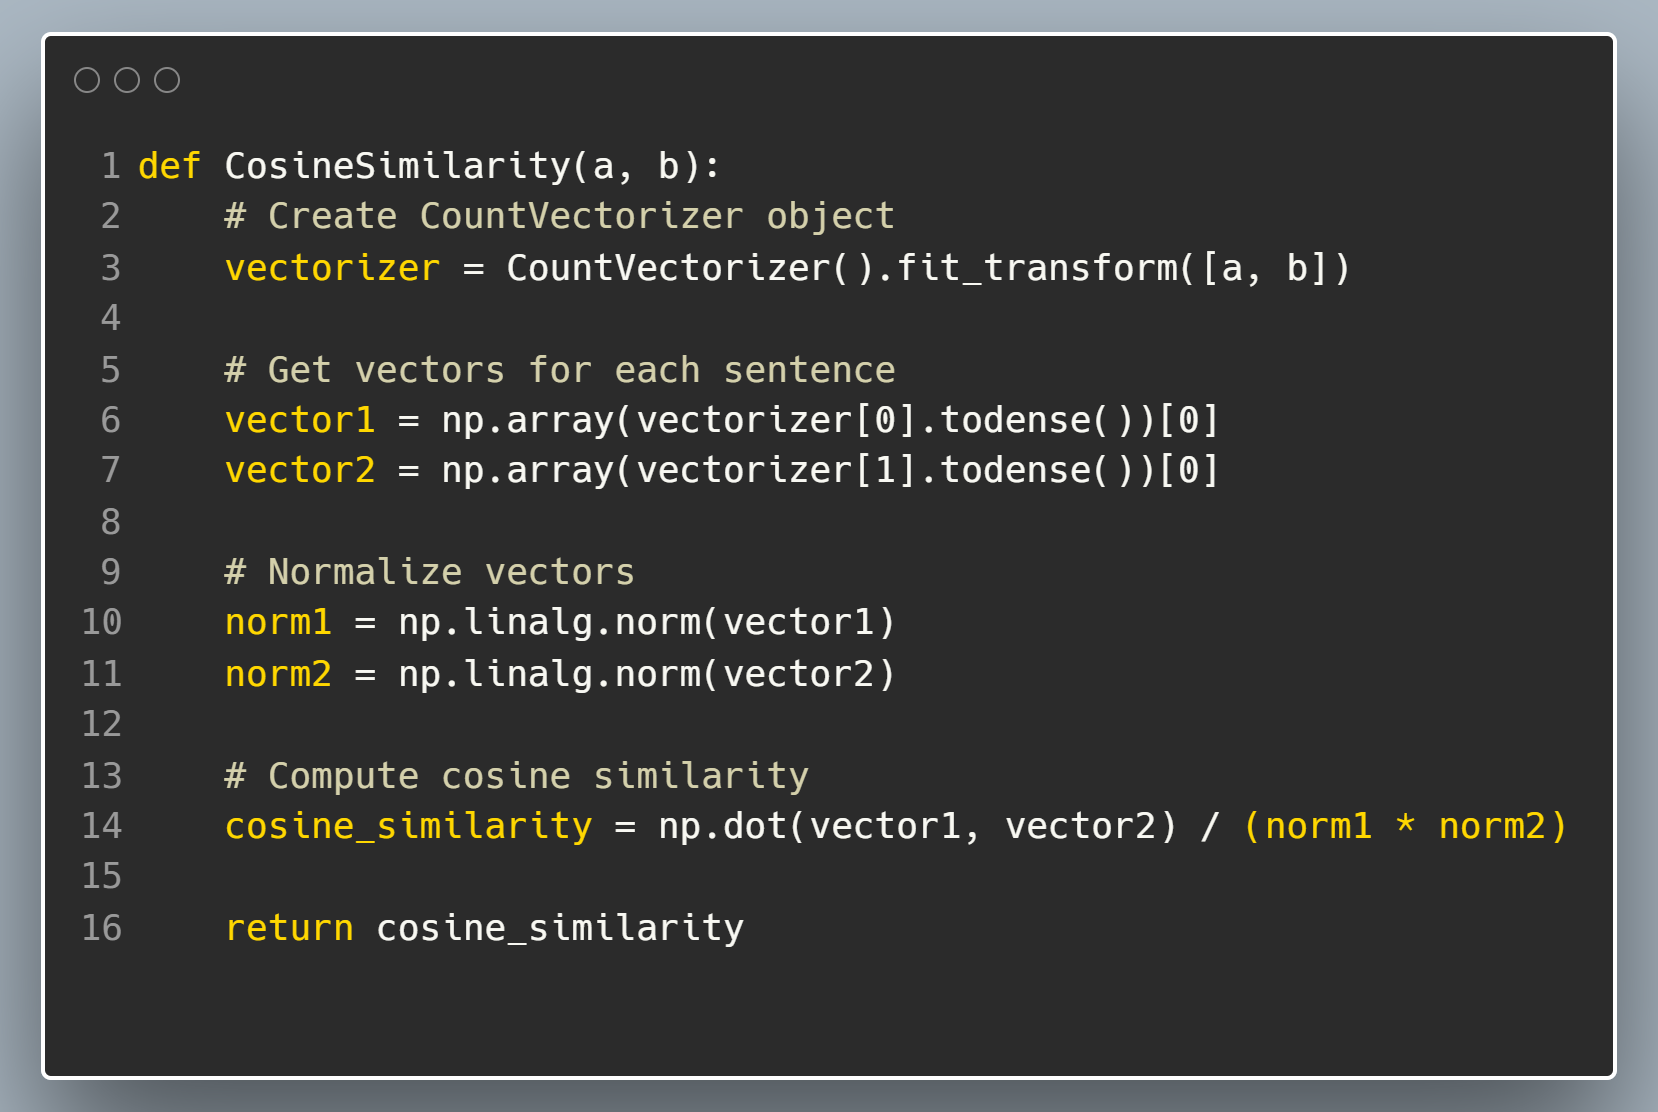
\includegraphics[width=0.6\textwidth]{images/cosine-similarity-code-snipet.png}
  \captionof{figure}{Cosine Similarity Code Snippet}
  \label{fig:cosine-similarity-code-snipet}
  \end{minipage}
  \\
  Figure \ref{fig:cosine-similarity-code-snipet} represents the snippet of the code which implements the theory. First, the CountVectorizer object is initialized from the Sklearn library. With this, we can convert the input string a (ChatGPT) and b (Google Search) to convert them into vectors of word counts. After that, we fit the vectorizer to the input strings and transform them into the vectors. From there the resulting vectors are normalized to ensure that the length of the vectors does not affect the similarity measure. Lastly, the cosine similarity between the two vectors is calculated using the dot product of the two vectors and dividing them by the product of their norms. 

\noindent
  \begin{minipage}{\linewidth}
  \centering
  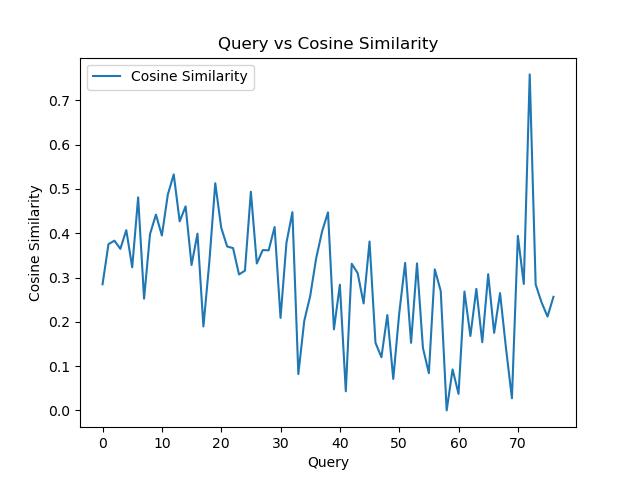
\includegraphics[width=0.65\textwidth]{images/cosine-similarity.png}
  \captionof{figure}{Query vs Cosine Similarity}
  \label{fig:cosine-similarity}
  \end{minipage}
  \\
  From the results, we can determine that the average cosine similarity value is 0.296, which indicates that the ChatGPT and Google Search from cosine similarity analysis have some degree of similarity, but they are far from identical. The maximum the cosine similarity went is 0.941, while the minimum it went is 0.0. This shows there are queries that are very similar and there are some which have no correlation with each other. The median value is 0.29617443887954614 which is very close to the average, meaning that there are not many extreme values. 

  \begin{table}[H]
    \centering
    \begin{tabular}{|c|c|c|c|c|c|c|}
      \hline
      average & max & min & median \\
      \hline
      \hline
      0.29629571650045594 & 0.9412657491818057 & 0.0 & 0.29617443887954614 \\
      \hline
    \end{tabular}
    \caption{Cosine Similarity Statistics}
    \label{tab:cosine_similarity_statistics}
  \end{table}

\paragraph{Jaccard Similarity}
Jaccard Index Coefficient or also known as Critical Success Index \cite{niwattanakul2013using}, is a measurement used to compute the similarity between two asymmetric binary variables. The Jaccard index is defined as the size of the intersection of the two sets divided by the size of the union of the two sets. This can be written in the below notation of two sets A and B.

\begin{equation}
  J(A,B) = \frac{|A \cap B|}{|A \cup B|}
\end{equation}
Jaccard Similarity will be 0 if the two sets tend to share no values, and 1 if both sets are identical. We can also use it to find the dissimilarity between the two sets, however in our case, we focus more on the similarity.
\noindent
  \begin{minipage}{\linewidth}
  \centering
  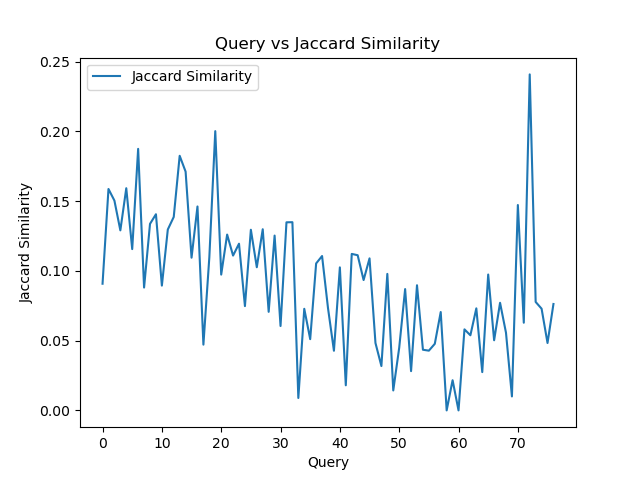
\includegraphics[width=0.7\textwidth]{images/jaccard-similarity.png}
  \captionof{figure}{Query vs Jaccard Similarity}
  \label{fig:jaccard-similarity}
  \end{minipage}
  \\

  % \noindent
  % \begin{minipage}{\linewidth}
  % \centering
  % 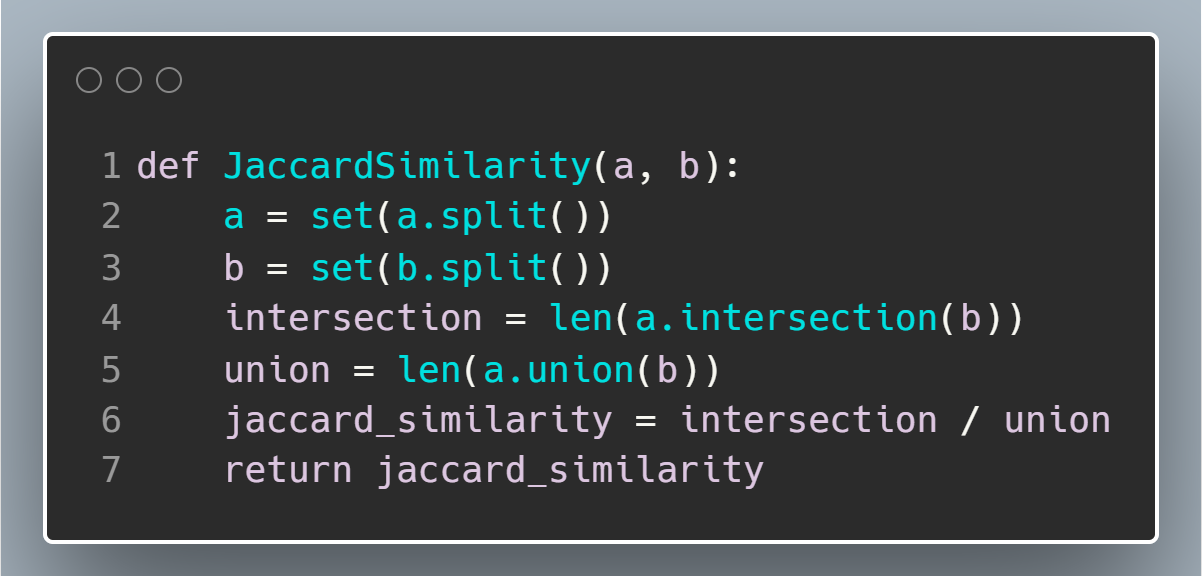
\includegraphics[width=0.7\textwidth]{images/jaccard-similarity-code-snipet.png}
  % \captionof{figure}{Jaccard Similarity Code Snippet}
  % \label{fig:jaccard-similarity-code-snipet}
  % \end{minipage}
  % \\

Hence from the evaluation we were able to determine that 9.09 \% of the elements in ChatGPT and Google Search are in common. The maximum Jaccard Similarity is 0.42, while the lowest was 0. The median of the Jaccard Similarity was 0.0784. Therefore, from Jaccard Similarity it can be seen that ChatGPT and Google search gave out very different results in this form of evaluation. Table \ref{tab:jaccard_similarity_statistics} shows the statistics of the Jaccard Similarity.

\begin{table}[H]
  \centering
  \begin{tabular}{|c|c|c|c|c|c|c|}
    \hline
    average & max & min & median \\
    \hline
    \hline
    0.09091836722083915 & 0.42 & 0.0 & 0.0784313725490196 \\
    \hline
  \end{tabular}
  \caption{Jaccard Similarity Statistics}
  \label{tab:jaccard_similarity_statistics}
\end{table}

\paragraph{Euclidean Similarity}
Euclidean Similarity \cite{elmore2001euclidean} is a measure used to determine the similarity or dissimilarity between two objects or data points in a Euclidean Space. This is calculated by the straight-line distance between two points in an n-dimensional space. The formula below describes Euclidean Similarity.

\begin{equation}
  d(p,q) = \sqrt{(q_1 - p_1)^2 + (q_2 - p_2)^2 + ... + (q_n - p_n)^2}
\end{equation}
The way in which we have implemented Euclidean Similarity is by first taking in two strings which are the ChatGPT result and the Google Search result. The function creates a CountVectorizer object which it fits in the two input strings. After that for each string, it gets a vector and normalizes it. Then it computes the Euclidean Distance between the two normalized vectors and returns the Euclidean similarity. 

The way in which Euclidean Similarity is calculated is by $ \frac{1}{1 + Euclidean Distance}$. As mentioned before the Euclidean Distance is the measure of the distance between two points in the multidimensional space. Euclidean Similarity is between 0 and 1, where 1 indicates that both the strings are identical, while 0 indicates that they are completely different. We use the libraries NumPy and sklearn to perform and simplify the calculations. The NumPy library is used for the vector normalization, while the sklearn is used to create the CountVectorizer. 

\noindent
  \begin{minipage}{\linewidth}
  \centering
  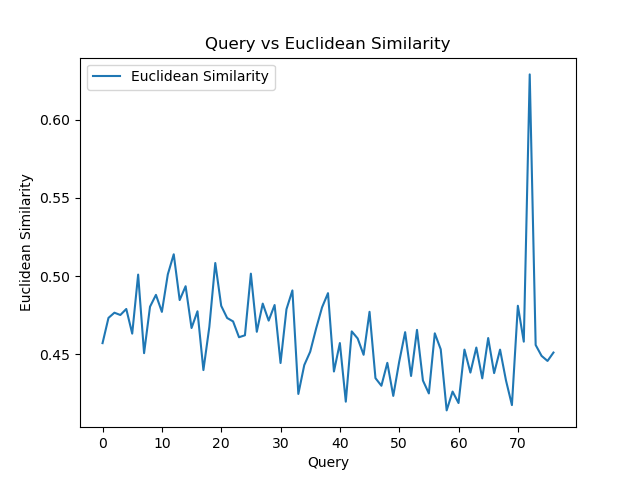
\includegraphics[width=0.7\textwidth]{images/euclidean-similarity.png}
  \captionof{figure}{Query vs Euclidean Similarity}
  \label{fig:euclidean-similarity}
  \end{minipage}
  \\
  From Figure \ref{fig:euclidean-similarity} there are several statistics that can be gathered. From these statistics, it can show that to some degree there is a similarity between the results returned by ChatGPT and Google search with an average similarity of 0.462. The maximum the similarity went was 0.745 while the lowest it went was 0. The median for Euclidean similarity is 0.457 which shows that the majority of the results are similar. Table \ref{tab:euclidean_similarity_statistics} shows the statistics of Euclidean Similarity.

\begin{table}[H]
    \centering
    \begin{tabular}{|c|c|c|c|c|c|c|}
      \hline
      average & max & min & median \\
      \hline
      \hline
      0.462 & 0.745 & 0.0 & 0.457 \\
      \hline
    \end{tabular}
    \caption{Euclidean Similarity Statistics}
    \label{tab:euclidean_similarity_statistics}
\end{table}

\paragraph{Pearson Correlaion}
Pearson Correlation Coefficient \cite{cohen2009pearson} is a measure of linear correlation between two sets of data. It is the ratio better the covariance of two variables with the product of their standard deviations. It is a normalized measurement of the covariance so that the result always has a value between -1 and 1. If the value is 1 it means that there is a total positive linear correlation, while if it is 0, it means that there is no correlation, and lastly, if it's -1, it means that there is a total negative correlation.

In order to calculate the Pearson Similarity, first as always, the with CountVectorizer objects were created to transform the two input strings into vectors. The vectors then get normalized, from which the Pearson correlation coefficient was calculated. This is done by using the Pearson Function from the scripy.stats library. The library uses the below equation to compute the coefficient.

\begin{equation}
  r = \frac{\sum_{i=1}^{n} (x_i - \bar{x})(y_i - \bar{y})}{\sqrt{\sum_{i=1}^{n} (x_i - \bar{x})^2} \sqrt{\sum_{i=1}^{n} (y_i - \bar{y})^2}}
\end{equation}
\noindent
  \begin{minipage}{\linewidth}
  \centering
  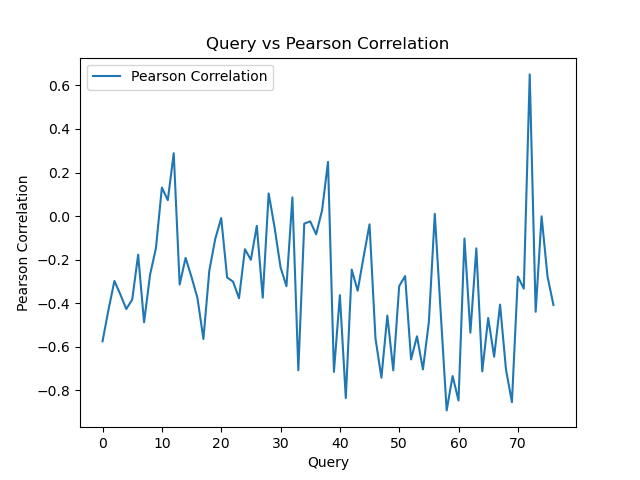
\includegraphics[width=0.7\textwidth]{images/pearson-correlation.png}
  \captionof{figure}{Query vs Pearson Correlaion}
  \label{fig:pearson-correlation}
  \end{minipage}
  \\

  From Figure \ref{fig:pearson-correlation} we can have some statistics which can be used later for analysis. We understand that the average correlation coefficient is -0.320, meaning that there is a weak negative correlation between the two sources. It means that the frequency of some certain terms or entities is increased in one entity while in another it is decreased. The maximum correlation coefficient which went was 0.949, but in the other, the minimum is -0.955 meaning that there are some which are very similar, while others which are different. The median is -0.342 which is close to the average, which again also indicates that there is a negative correlation between the sources. Overall, it can be seen that there is some degree of correlation between ChatGPT and Google results, but their strength and direction vary depending on the comparison being made.

\begin{table}[H]
    \centering
    \begin{tabular}{|c|c|c|c|c|c|c|}
      \hline
      average & max & min & median \\
      \hline
      \hline
      -0.320 & 0.949 & -0.955 & -0.342 \\
      \hline
    \end{tabular}
    \caption{Pearson Correlation Statistics}
    \label{tab:cosine_similarity_statistics}
\end{table}

\subsubsection{Sentiment Analysis}
Sentiment Analysis \cite{medhat2014sentiment} is a very powerful technique that is used in natural language processing to determine different emotional tones behind a body of text. Such analysis involved analyzing the text to determine whether it is representing a positive, negative, or neutral sentiment. This analysis is helpful for our data, as it gives us a better understanding of what sentiment both Google and ChatGPT results give. We get the result between 0 and 1, 0 meaning the sentiment doesn’t exist while 1 meaning the whole sentence is that sentiment. What we expect from both is to give neutral results, as the results that the user usually seeks, want neutral answers. Both for Google and ChatGPT it will be tricky, as Google shows results written by people where sentiment can easily creep in, while ChatGPT generates its responses automatically.

\noindent
\begin{minipage}{\linewidth}
\centering
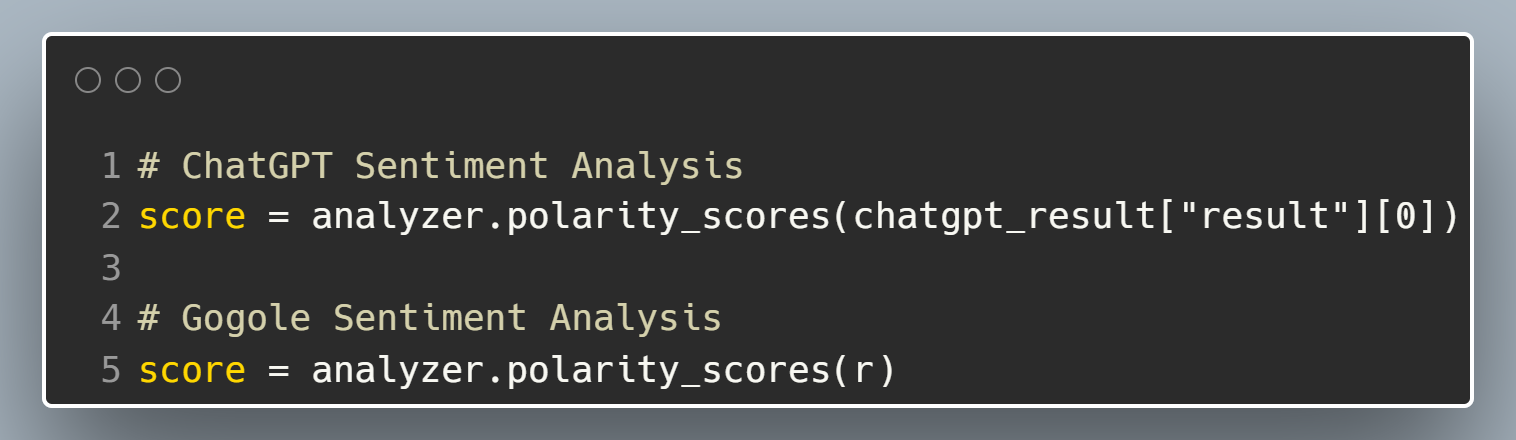
\includegraphics[width=0.7\textwidth]{images/sentiment-analysis-score-code-snipet.png}
\captionof{figure}{Sentiment Analysis Code Score Snippet}
\label{fig:sentiment-analysis-score-code-snipet}
\end{minipage}

The sentiment analysis is performed on data which we collected, which is the Google Results, and ChatGPT Results. We use the SentimentIntensityAnalyzer from nltk.sentiment module to analyze each sentence of the data. We then use the polarity score method to obtain scores for each sentence. The sentiment score includes, negative, neutral, and positive. The code snippet in Figure \ref{fig:sentiment-analysis-score-code-snipet} shows how the score was obtained.

\noindent
\begin{minipage}{\linewidth}
\centering
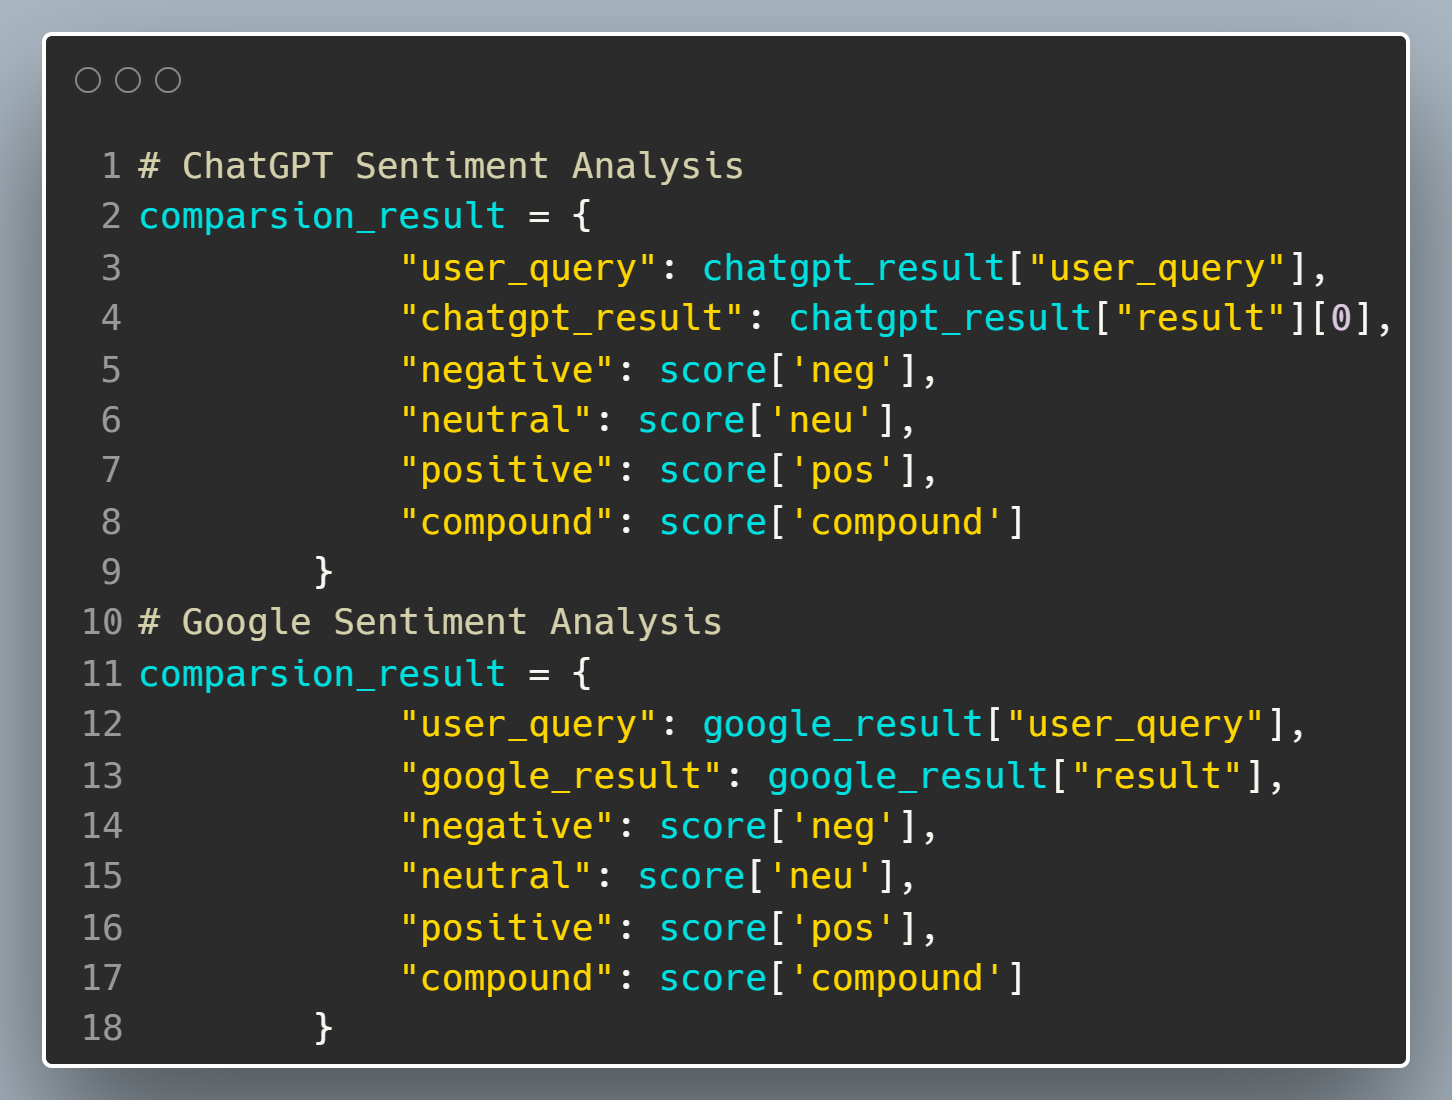
\includegraphics[width=0.7\textwidth]{images/sentiment-analysis-data-code-snippet.png}
\captionof{figure}{Sentiment Analysis Data Code Snippet}
\label{fig:sentiment-analysis-data-code-snippet}
\end{minipage}

Figure \ref{fig:sentiment-analysis-data-code-snippet} it shows the data structure which was used to get the results. It was initially collected in JSON and then transformed into CSV for consistency. 

\begin{figure}[H]
  \centering
  \subfigure[Negative Sentiment Analysis Google]{
    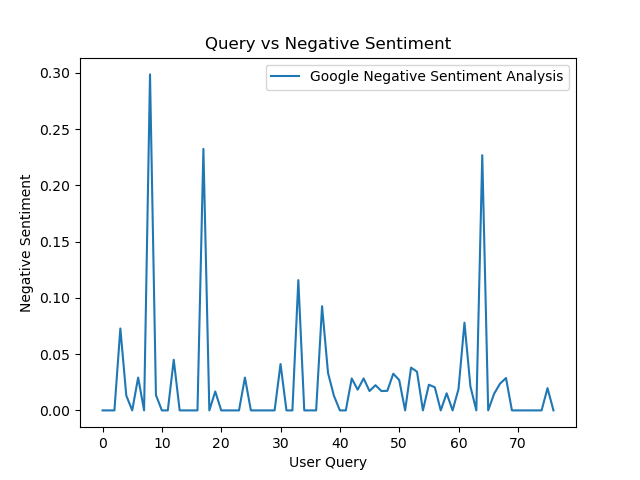
\includegraphics[width=0.4\textwidth]{images/negative-sentiment-analysis-google.png}
    \label{fig:negative-sentiment-analysis-google}
  }
  \hfill
  \subfigure[Positive Sentiment Analysis Google]{
    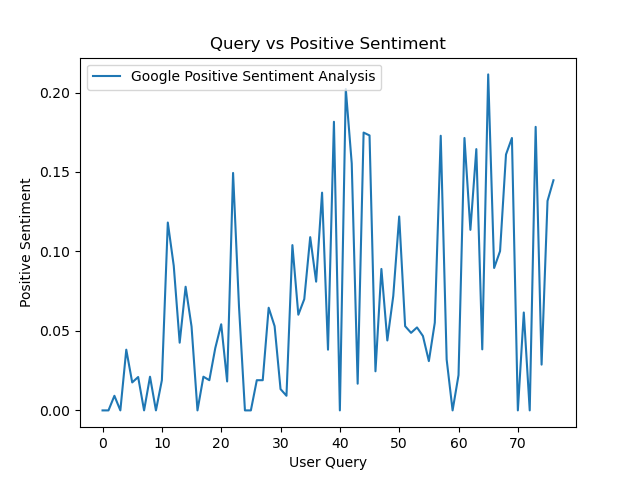
\includegraphics[width=0.4\textwidth]{images/positive-sentiment-analysis-google.png}
    \label{fig:positive-sentiment-analysis-google}
  }
  \hfill
  \subfigure[Neutral Sentiment Analysis Google]{
    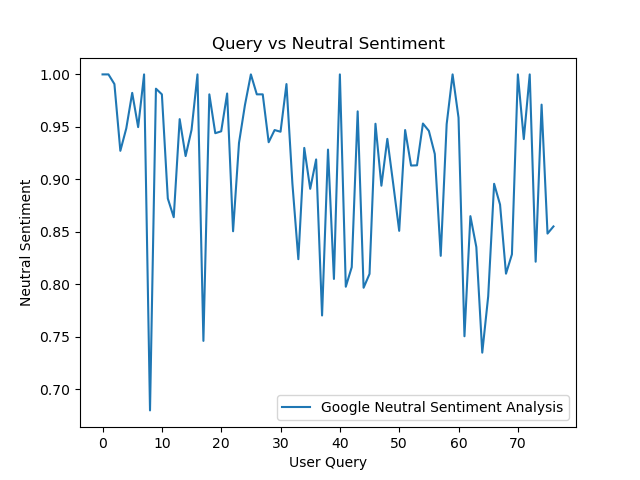
\includegraphics[width=0.4\textwidth]{images/neutral-sentiment-analysis-google.png}
    \label{fig:neutral-sentiment-analysis-google}
  }
  \caption{Sentiment Analysis Google}
  \label{fig:sentiment-analysis-google}
\end{figure}

Figure \ref{fig:sentiment-analysis-chatgpt} represent the Sentiment Analysis of Google. As most of the text is considered Neutral with the average being 0.91. The average for negative and positive sentiment is 0.03 and 0.02 respectively, with the highest for both went was 0.53 and 0.45. Also, if the mean is noticed for the neutral sentiment, it is 1, which is close to the Average. This analysis can show that Google results tend to have more neutral sentiment possibly resulting in less biased and more objective information retrieved.

\begin{figure}[H]
  \centering
  \subfigure[Negative Sentiment Analysis ChatGPT]{
    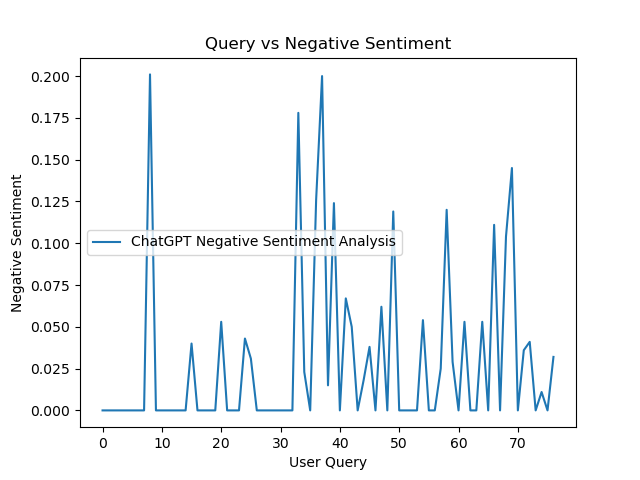
\includegraphics[width=0.4\textwidth]{images/negative-sentiment-analysis-chatgpt.png}
    \label{fig:negative-sentiment-analysis-chatgpt}
  }
  \hfill
  \subfigure[Positive Sentiment Analysis ChatGPT]{
    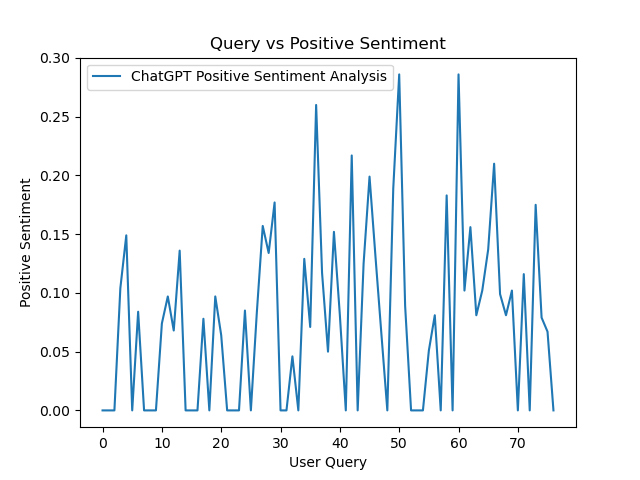
\includegraphics[width=0.4\textwidth]{images/positive-sentiment-analysis-chatgpt.png}
    \label{fig:positive-sentiment-analysis-chatgpt}
  }
  \hfill
  \subfigure[Neutral Sentiment Analysis ChatGPT]{
    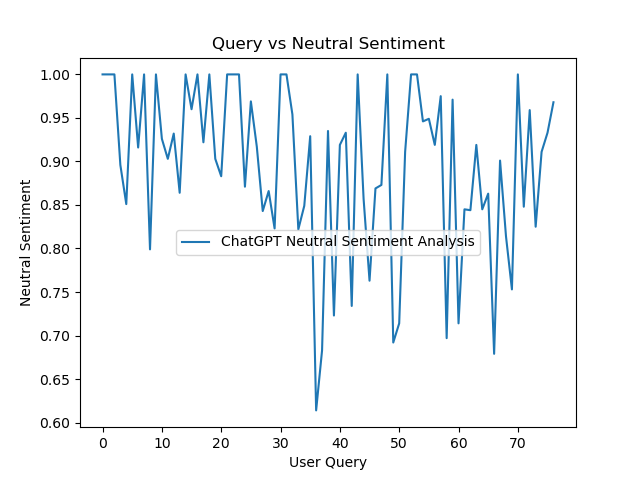
\includegraphics[width=0.4\textwidth]{images/neutral-sentiment-analysis-chatgpt.png}
    \label{fig:neutral-sentiment-analysis-chatgpt}
  }
  \caption{Sentiment Analysis ChatGPT}
  \label{fig:sentiment-analysis-chatgpt}
\end{figure}

Figure \ref{fig:sentiment-analysis-chatgpt} represent the Sentiment Analysis of ChatGPT. Similarly, to Google, most of the results from ChatGPT come under Neutral Sentiment with an average of 0.89. The highest the neutral sentiment has gone is 1, while the lowest it has gone is 0.61. The median as well for the ChatGPT is 0.92. Also, the negative and positive sentiment is 0.03 and 0.08 respectively, which is very close to what Google sentiments are as well. 

At last, when we compare the results of ChatGPT and Google Search with each other we can notice a few things. For instance, even though ChatGPT average is slightly lower than Google’s for Neutral Sentiment it can be noticed that Google went as low as 0.47 while ChatGPT stayed at 0.61. Also, if you see Negative Sentiment as well, while the average for ChatGPT is slightly higher, its max is nearly half as low as compared to Google's Negative Sentiment. The same goes for the Positive Sentiment as well, showing that Google tends to have more extreme cases. From this we can conclude that on average both Google’s and ChatGPT’s results are neutral, however, in some cases, there are not, it's more likely for Google to have an extremely negative or positive result as compared to ChatGPT's results. Figures \ref{fig:negative_sentiment_analysis}, \ref{fig:positive_sentiment_analysis}, and \ref{fig:neutral_sentiment_analysis} show the average, median, max, and min for each of the sentiment analysis.



\begin{figure}[H]
  \centering
  \subfigure[ChatGPT]{
    \begin{tabular}{|c||c|}
      \hline
      \textbf{Average} & 0.03 \\
      \hline
      \textbf{Median} & 0.00 \\
      \hline
      \textbf{Max} & 0.20 \\
      \hline
      \textbf{Min} & 0.00 \\
      \hline
    \end{tabular}
    \label{tab:negative_sentiment_analysis_chatgpt}
  }
  \subfigure[Google]{
    \begin{tabular}{|c||c|}
      \hline
      \textbf{Average} & 0.02 \\
      \hline
      \textbf{Median} & 0.00 \\
      \hline
      \textbf{Max} & 0.53 \\
      \hline
      \textbf{Min} & 0.00 \\
      \hline
    \end{tabular}
    \label{tab:negative_sentiment_analysis_google}
  }
  \caption{Negative Sentiment}
  \label{fig:negative_sentiment_analysis}
\end{figure}

\begin{figure}
  \centering
  \subfigure[ChatGPT]{
    \begin{tabular}{|c||c|}
      \hline
      \textbf{Average} & 0.89 \\
      \hline
      \textbf{Median} & 0.92 \\
      \hline
      \textbf{Max} & 1.00 \\
      \hline
      \textbf{Min} & 0.61 \\
      \hline
    \end{tabular}
    \label{tab:neutral_sentiment_analysis_chatgpt}
  }
  \subfigure[Google]{
    \begin{tabular}{|c||c|}
      \hline
      \textbf{Average} & 0.91 \\
      \hline
      \textbf{Median} & 1 \\
      \hline
      \textbf{Max} & 1.00 \\
      \hline
      \textbf{Min} & 0.47 \\
      \hline
    \end{tabular}
    \label{tab:neutral_sentiment_analysis_google}
  }
  \caption{Neutral Sentiment}
  \label{fig:neutral_sentiment_analysis}
\end{figure}

\begin{figure}
  \centering
  \subfigure[ChatGPT]{
    \begin{tabular}{|c||c|}
      \hline
      \textbf{Average} & 0.08 \\
      \hline
      \textbf{Median} & 0.08 \\
      \hline
      \textbf{Max} & 0.29 \\
      \hline
      \textbf{Min} & 0.00 \\
      \hline
    \end{tabular}
    \label{tab:positive_sentiment_analysis_chatgpt}
  }
  \subfigure[Google]{
    \begin{tabular}{|c||c|}
      \hline
      \textbf{Average} & 0.07 \\
      \hline
      \textbf{Median} & 0.00 \\
      \hline
      \textbf{Max} & 0.45 \\
      \hline
      \textbf{Min} & 0.00 \\
      \hline
    \end{tabular}
    \label{tab:positive_sentiment_analysis_google}
  }
  \caption{Positive Sentiment}
  \label{fig:positive_sentiment_analysis}
\end{figure}



\section{Machine Learning Model}
\label{sec:machine_learning_model}
One of the tools which this project aims to develop is a tool that can tell if a result from a search query is relevant or not. This is a very ambitious goal, and to achieve that we thought it is wise to use Machine Learning. Along with the data which were collected from children, Professor Monica and her team were able to go manually through each result from Google Search to determine if it is relevant or not relevant. Hence, we thought it would be wise to use that data and train a machine learning module that can learn different patterns and teach itself to recognize if some result is relevant or not. 

\subsection{Creation of ML Model}
The model is trained on Logistic Regression \cite{lavalley2008logistic} which is best suited for this problem as it is usually used to solve binary classification problems. The goal of logistic regression is to predict a binary outcome such as yes or no and in our case it is relevant or not relevant. This generalized linear model uses a logistic function to model different relationships between the input variables and the output variables. Logistic Regression is trained to find the coefficients which maximize the likelihood of the observed data with the given mode. 

Hence the approach for this was to first to read the data and split the data into target and feature. The feature in our case is the user query and the snippet columns where the results of the user query are. The target is the source column which would give a binary result; relevant or not relevant. Firstly, the text data in the features is pre-processed using CountVectorizer which would convert the text data into a matrix of different token counts. From there the data is split into training and testing sets using the train test split. The reason why the split is done is so that the performance of the Machine Learning Module can be evaluated. From there we use the logistic regression model to train itself on the trained data and then get evaluated against the test data. 

\subsection{Evaluation of ML Model}
\begin{table}[H]
  \centering
  \begin{tabular}{|c||c|c|c|c|}
    \hline
    & precision & recall & f1-score & support \\
    \hline
    \hline
    NR & 0.81 & 0.98 & 0.89 & 132 \\
    R & 0.83 & 0.25 & 0.38 & 40 \\
    accuracy & \null & \null & 0.81 & 172 \\
    macro avg & 0.82 & 0.62 & 0.64 & 172 \\
    weighted avg & 0.82 & 0.81 & 0.77 & 172 \\
    \hline
  \end{tabular}
  \caption{Classification Report}
  \label{tab:classification_report}
\end{table}

Table \ref{tab:classification_report} shows the performance of the model. As can be seen, the precision of NR and R is 0.81 and 0.83 respectively which is quite high. However, the F1 score should be looked at more properly as it takes into account both precision and recall. F1 score is the harmonic mean of precision and recall which ranges from 0 and 1. As can be seen for NR the F1 score is 0.89 however the F1 score for R is 0.38 which is quite low. 

However, these results don’t tell the full evaluation as the main problem here is that the data is simply too less to make a proper model. When comparing these results from results gather from ChatGPT out of 77 queries it said that only 1 is relevant and the rest is non-relevant. Hence this module is not practical, but it is a good starting point to develop when more data is collected.


\section{Validation}
\label{sec:validation}
\subsection{Analysis of Results}
In the end, after all the collection of data and evaluation has been done, we can finally look at what all the analysis has shown to us. What we have realized is that results from both Google Search and ChatGPT differ a lot from each, and this was proven by all the different Similarity Analyses which we ran on them. This claim is supported by the fact the length of their response varies a lot. The average character per response for Google is 151, while the average character per response for ChatGPT is 342, nearly 3 times more. With the main caveat that Google provides a SERP made of short snippets while ChaGPT gives just one cohesive answer.

\noindent
\begin{minipage}{\linewidth}
\centering
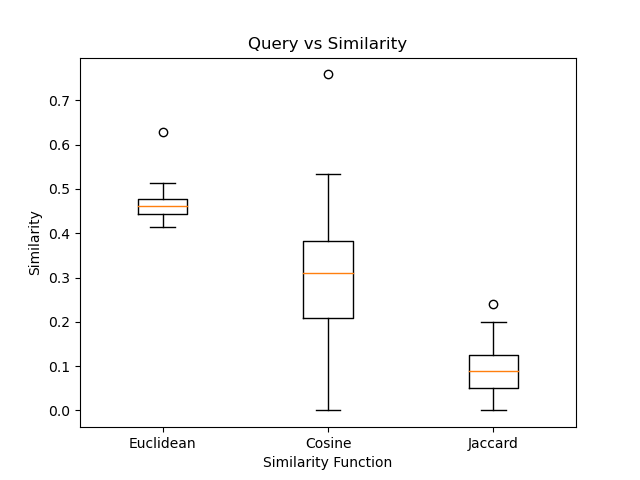
\includegraphics[width=0.7\textwidth]{images/similarity-analysis-box.png}
\captionof{figure}{Similarity Analysis}
\label{fig:similarity_analysis}
\end{minipage}

In Figure \ref{fig:similarity_analysis}, we can see a box graph visualizing Cosine, Jaccard, and Euclidean Similarity. This graph is helpful for us to understand the distribution of the different similarities as they have the same scale. It can also be noticed that there were some cases where in the extreme end both Euclidean and Cosine Similarity showed a high value. Euclidean Similarity had an average higher average as compared to Cosine and Jaccard Similarity. This is because Euclidean Similarity is more sensitive to outliers as compared to Cosine and Jaccard Similarity. On the other hand, Jaccard Similarity had the lowest average as it is more sensitive to the length of the response. Cosine Similarity is the most spread out among the three.

However, having more response does not mean that what ChatGPT provide is richer with its response. Instead, when we analyze the Named Entity Recognition (NER) of both Google and ChatGPT we can have a better understanding of the richness of their responses. From the results of NER Analysis, we can see that the top 5 entities for both Google Search and ChatGPT and nearly the same, however where they are different is the number of times they occur. The average number of entities per response is 18.2 for Google, while for ChatGPT it is 6.11. This means that the quality of information that Google provides is much richer with important facts and information as compared to ChatGPT. Hence despite having a much longer response as compared to Google, ChatGPT’s responses lack the variation and amount of entities in their response. 

Another interesting thing that we found out was that the sentiment of the responses from both Google and ChatGPT are quite similar. The average sentiment of Google is 0.07, while the average sentiment of ChatGPT is 0.08. This looks to show that the responses from both Google and ChatGPT are quite neutral. However, when we look at the distribution of the sentiment of the responses from both Google and ChatGPT we can see that the distribution of the sentiment of the responses from Google is more spread out as compared to ChatGPT. This means that the responses from Google are more diverse as compared to ChatGPT. Hence, when it comes to the cases in which the response for Google is not neutral, their response could either have more positive sentiment or negative sentiment as compared to ChatGPT. This means that in some cases there can be possibilities of some biased involved in the response.

At last, when we look at the performance of the Machine Learning Module which we developed, we can see that the performance of the model is quite good when evaluated against test data. The F1 score for the relevant results is 0.38 which is quite low, however, the F1 score for the non-relevant results is 0.89 which is quite high. This means that the model is quite good at predicting the non-relevant results, however, it is not good at predicting the relevant results. On the other when we use this model with some other data, we can again see a clear limitation since it predicts most of the responses as Relevant while once while it predicts non-Relevant. This is because the data which was used to train the model was not enough. Hence, the model is not practical, but it is a good starting point to develop when more data is collected. Also, it is not essential to use such type of data, but maybe some other data could be used which is finer tuned for ChatGPT as the previous one had responses from Google.

% At the end, we understand that with it can be concluded that for now the better option to use is Google Search as it provides more relevant and rich information as compared to ChatGPT. However, this does not mean that ChatGPT is not useful, as it can be used to provide some additional information which Google Search does not provide. Hence, it can be used as a complementary tool to Google Search. With future work, we can look at how we can use ChatGPT to provide some additional information which Google Search does not provide.

In the end, when we come back to the research question \textbf{"Are the new conversational AI models safer for children to interact with, or do the traditional search engine still hold an edge over the new technology?"}, we can see that the answer is not as simple as it seems to be. However, we were still able to see enough differences to make a conclusion that currently Google Search is a better option as compared to ChatGPT for children. This is because Google Search provides more relevant and rich information as compared to ChatGPT, but this does not mean that ChatGPT has not performed well. Currently, ChatGPT can very well be used as a complementary tool to Google Search. With future improvements to the technology ChatGPT and other conversational AI, models can very well be used as a replacement for Google Search and be a better option for children to interact with. Conversational AI models have the ability to mimic human conversations and can be used as an interactive tool for children to learn in the future. 
\subsection{Limitations}
Throughout the project, there were several limitations that came across. The first limitation was the data which was used in this project. Even though the data was not as old, it still can be considered outdated due to the fast-paced advancement of technology, especially among young users. Another factor about the data was its limited quantity, which had a huge impact on the machine learning model. Much more data was needed to have a much more robust machine learning model. 

Another limitation of this project was that the scope of this project was a bachelor project. Such research-oriented project demands more resources and time. Along with that a lot of time was invested in learning how to use the tools so that proper results can be produced.

\begin{table}[H]
  \centering
  \begin{tabular}{|l|l|l|l|l|}
    \hline
    \textbf{Statistic} & \textbf{Average} & \textbf{Max} & \textbf{Min} & \textbf{Median} \\ \hline
    Cosine Similarity & 0.296 & 0.941 & 0 & 0.296 \\ \hline
    Euclidean Similarity & 0.462 & 0.744 & 0 & 0.457 \\ \hline
    Jaccard Similarity & 0.091 & 0.42 & 0 & 0.078 \\ \hline
    Pearson Correlation & -0.321 & 0.949 & -0.955 & -0.342 \\ \hline
    Google Query Length & 151.44 & 162.2 & 132.8 & 153.8 \\ \hline
    ChatGPT Query Length & 343.81 & 1321 & 81 & 237 \\ \hline
    Google NER & 18.22 & - & - & - \\ \hline
    ChatGPT NER & 6.12 & - & - & - \\ \hline
    ChatGPT Negative Sentiment & 0.03 & 0.20 & 0.00 & 0.00 \\ \hline
    ChatGPT Neutral Sentiment & 0.89 & 1.00 & 0.61 & 0.92 \\ \hline
    ChatGPT Positive Sentiment & 0.08 & 0.29 & 0.00 & 0.08 \\ \hline
    Google Negative Sentiment & 0.02 & 0.53 & 0.00 & 0.00 \\ \hline
    Google Neutral Sentiment & 0.91 & 1.00 & 0.47 & 1.00 \\ \hline
    Google Positive Sentiment & 0.07 & 0.45 & 0.00 & 0.00 \\ \hline
  \end{tabular}
  \caption{Summary of Results}
  \label{tab:summary_of_results}
\end{table}

In Table \ref{tab:summary_of_results}, we can see a summary of the results which we have discussed above. This table is helpful for us to understand the distribution of the different results as they have the same scale.


Finally, the last limitation was that the technology being analyzed, especially the conversational models is very fast-paced. A lot is being in development at such technology from both the technical perspective but also the rules and regulations perspective. This is a very new technology to even this day many new findings are being found. However, despite this project having a small scale it provides a fresh perspective to such a field. This project aims to be a stepping stone for another project to launch itself. This project provides tools that facilitate analysis and comparison between traditional search engines and bleeding-edge conversational models. 

\subsection{Future Work}
There are several ways that this project can be extended. For instance, with more data, the whole project can become much more robust, especially the machine learning module to detect relevant and non-relevant results. Another way in which this project can be extended is by using the tools developed for other projects related to this field. The projects can be such as analyzing the performance of different conversational models, or analyzing the performance of different search engines and comparing them to the current standards. The field of conversational models has brought us a new and exciting way of absorbing information; however, such fast-paced technology always has threats to it. With the tools developed throughout the duration of this project, they can be used to analyze such technologies. The tools are all based on the latest technologies with well-written documentation to support them. It is designed to be adaptable to different projects and goals. Involving real users in the study would make it more effective and complex at the same time.

%%%%%%%%%%%%%%%%%%%%%%%%%%%%
\newpage
\section*{Acknowledgements}
I would like to thank Prof. Dr. Landoni Monica for allowing me to work on this project and for providing me with her guidance and support throughout the duration of this project. I would also like to thank family and friends for their support and encouragement throughout the duration of this project. Finally, I would like to thank the Università della Svizzera Italiana for providing me with the opportunity to work on this project.

\newpage
%%%%%
\bibliographystyle{abbrv}
\bibliography{references}

\end{document}
}
